% Kelompok Willem Jansz Bleau
% Hanna Tasya ( 1154091 )
% Aji Muhammad Farhan ( 1154046 )
% Dhea Amelia ( 1154123 )
% Tias Maulana ( 1154122 )
% Yusri Rizal ( 1154072 )


\section{Biografi Willem Jansz Blaeu}
Dalam biografi nya tentang willwm jansz Blaeu 1932, tapi tidak mungkin F. C. Wieder sudah merujuk pada ada nya lembaran tangan bawah 
dari peta ini di Museum Nasional Germanisches di Nurnberg. Sampai saat ini, investigasi di dasarkan pada lembar satu ini di Nurnberg 
dan deskripsi singkat dari Wieder yang menyebut peta ini sebagai monumen ukiran dan karya seni Belanda yang di ciptakan oleh seorang 
pria hebat dan berbudaya, sebuah monumen ilmiah yang luar biasa dari awal masa kolonial. Sementara penulis saat ini sedang belajar 
di Rijksmuseum Nederlands Scheepvaart-Museum di Amsterdam, dia membolak-balik dua kotak foto peta yang diperoleh dalam sebuah lelang yang di adakan pada tahun 1958. 
'Betapa terkejut nya dia menemukan di antara foto-foto ini yang terpaku pada kardus gambar kecil (9 x 13cm) peta dinding dunia 
pada proyeksi Mercator oleh Willem Jansz Bleau dari tahun 1606-1607. Ini memberi kesan visual tentang keindahan asli bintang yang hilang ini. 
Gambar 1) dan memungkinkan deskripsi detail dari peta itu sendiri dan pengaruhnya terhadap peta dunia lainnya. 
Penulis buku ini mencoba membuat foto kecil yang di perbesar oleh Layanan Topografi di Delft sampai ukuran seperti itu 
sehingga garis pantai bisa menjadi lebih jelas dan huruf iegen terbaca. Pembesaran ini membuat kontur pantai lebih jernih namun teks tetap tidak jelas. 

\cite{Schilder1979Willem}

\begin{figure}[ht]
	

\centerline{\includegraphics[width=1\textwidth]{figures/willem_jansz_blaeu.png}}
	

\caption{Willem Janzs Blaeu}
	

\labelwillem_jansz_blaeu


\end{figure}



\subsection{karya individual willem jansz bleau}
willem jansz Bleau karya kartografi individual yang di terbitkan paling awal di Blaeu mencakup tiga peta dinding dunia, 
masing - masing di gambar dalam proyeksi yang berbeda. Dengan menyediakan berbagai macam bahan, yang telah disediakan untuk proyeksi tersebut. 
willem jansz bleau mencoba memenuhi semua permintaan pelanggan nya sambil bersaing dengan penerbit peta lain nya di amsterdam. 


pada paten dua belas tahun yang di berikan kepada cornelis claeszoon untuk dapat mempublikasi peta dunia 1592 oleh plancius, peta datar silinder 20 lembar,
yang telah kadaluarsa pada tahun 1604. peta oleh plancius ini merupakan tengara penting dalam pengembangan kartografi dan membangkitkan kekaguman 
terhadap orang � orang di zaman pembuatan peta, dimana peta di buat untuk alasan komersial, willem jansz bleau Buru - buru memproyeksikan agar 
peta dunia ini di ukir kembali oleh josua van den dan di ubah dengan penemuan � penemuan terbaru. 


\section{Peta dinding diterbitkan}
Pada periode yang sama, willem jansz bleau. Dianggap menerbitkan peta dinding dunia dengan proyeksi stereografik. 
peta dinding di dua belahan otak ini di terbitkan pada tahun 1605 oleh willem jansz bleau. dan pada akhirnya, untuk memenuhi semua kebutuhan pelanggannya, willem jansz bleau juga memutuskan untuk menerbitkan peta dunia mengenai proyeksi mercator. 
peta dinding ini di proyeksikan akan berpengaruh pada peta dunia lainnya yang akan dibahas di bawah ini. tidak ada salinan lengkap peta ini yang bertahan. sementara j. keuning sedang katalogisasi f. c. Wieder 's tentang warisan museum maritiem' 
prins hendrik 'di rotterdam, ia menemukan di antara dokumen - dokumen deskripsi dari peta dunia ini pada proyeksi mercator. 
deskripsi ini, yang di tulis oleh f. c. wieder, di masukkan secara lengkap di j. Keuning biografi bleau. 

\cite{campbell1976descriptive}

\begin{figure}[ht]
	

\centerline{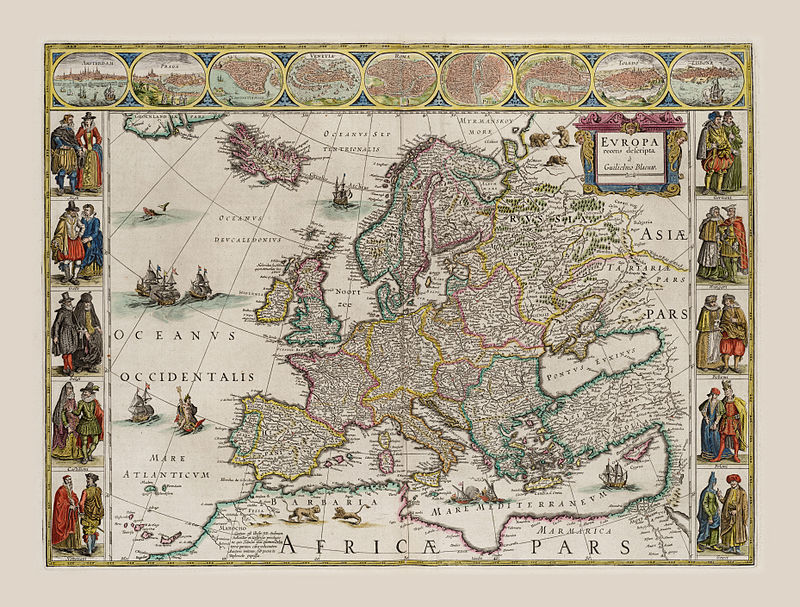
\includegraphics[width=1\textwidth]{figures/petadinding.jpg}}
	

\caption{Peta Dinding}
	

\label{petadinding}

\end{figure}

gambar ini \ref{petadinding.jpg} merupakan peta yang dibuat oleh Willem Blaeu pada tahun 1640
 
Wieder Menjual Petanya dan Berhasil ditemukanya peta dinding oleh WillemJansz Bleau .Namun, artikel tersebut tidak menyebutkan lokasi peta dinding berada. 
Selama perang dunia kedua wieder menjual koleksi peta itu sendiri di berlin dimana ia hilang di dalam kekacauan. 
Sehingga sangat mungkin koleksi ini termasuk peta dinding dunia. tentang proyeksi mercator 1606 - 1607, 
karena dalam salinan pribadi kartografi monumenla ini (sekarang di pelihara di perpustakaan negara bagian barat berlin) 
dr. wieder di tandai dalam manuskrip - dengan catatan : 'sekarang peta ini selesai'. 


Di dalam biografi nya tentang willem jansz Blaeu 1932 , tapi tidak mungkin F. C. Wieder sudah merujuk pada adanya lembaran tangan dari 
peta ini di Museum Nasional Germanisches di Nurnberg. Sampai saat ini, investigasi di dasarkan pada lembar satu yang ini di Nurnberg dan deskripsi singkat dari Wieder yang menyebut peta ini sebagai monumen ukiran 
dan karya seni Belanda yang di ciptakan oleh seorang pria hebat dan berbudaya, sebuah monumen ilmiah yang luar biasa dari awal masa �colonial'. 
Sementara penulis saat ini sedang belajar di Rijksmuseum Nederlands Scheepvaart-Museum di Amsterdam, 
dia membolak-balik dua kotak foto peta yang di peroleh dalam sebuah lelang yang di adakan pada tahun 1958. 
'Betapa terkejut nya dia menemukan di antara foto-foto ini yang terpaku pada kardus gambar kecil ( 9 x 13 cm ) 
peta dinding dunia pada proyeksi Mercator oleh Willem Jansz Bleau dari tahun 1606 - 1607. 
Ini memberi kesan visual tentang keindahan asli bintang yang hilang ini. 
Gambar 1) dan memungkinkan deskripsi detail dari peta itu sendiri dan pengaruh nya terhadap peta dunia lain nya. 
Penulis buku ini mencoba membuat foto-foto kecil yang di perbesar oleh Layanan Topografi di Delft sampai ukuran seperti itu 
sehingga garis pantai bisa menjadi lebih jelas dan huruf iegen terbaca. 
Pembesaran ini membuat kontur pantai lebih jernih namun teks tetap tidak jelas. 
Untung nya, dengan mencari jalan ke berbagai peta dunia yang berasal dari Willem Jansz Bleau. 'peta dinding dia berhasil di patenkan. 

\cite{campbell1976descriptive}

\subsection{Karya Willem Blaeu}
Selama hampir 70 tahun, biografi Baudet Willem Jansz Bleau Maior sudah menjadi sumber utama untuk pengetahuan kita 
tentang kehidupan dalam karya willem jansz Blaeu's. Karena, bagaimana pun kurang nya sumber�sumber yang tersedia di tahun-tahun 
sebelum nya sudah di tangani sangat ringkas dalam karya tersebut. 
Ini khusus nya adalah kebenaran hubungan Brahe's dengan Tycho Brahe dan pelatihan yang diterima oleh Joll Ander muda dibawah bimbingan Brahe's pafa Hven. 
Pelatihan ini diketahui, dalam banyak cara untuk menentukan penting nya pekerjaan nanti nya dia di tanah sendiri. 
Pada tahun 1914 kehidupan dan pekerjaan willem jansz Baleu's akan diteliti dari awal oleh Stevenson, 
kalian ini dengan referensi khusus untuk karya nya, peta penting dunia 1605. Pekerjaan tidak berisi informasi lain yang bener-bener 
baru tentang hubungan willwm jansz Blaeu's dengan Brabe. Sejak hari Baudet's bagaimanapun, 
pengetahuan kita tentang kehidupan dan penelitian Brahe's sudah sangat meningkat. 
Dan telah memiliki sedikit bagian dalam hal ini. Pada tahun 1980 dreyer di terbitkan sejauh biografi paling rinci dan terbaik dari Brabe.  
Dreyer, salah satu sejarawan pembimbing astronomi di waktu kita dan dane, 
pada khusus nya di lengkapi untuk kumpulan karya Brahe's dan pada 1913 ia terbit di edisi jilis pertama dari Opera Omnia. 
Dua tahun setelah kematian nya, pada tahun 1928 pekerjaan selesai. 
Artinya dari koleksi surat ini dapat di tetapkan beberapa fakta lebih lanjut untuk tetap di Blaeu Hven dan pandangan sebelum nya di koreksi. 
Untuk jenis pengetahuan pelatihan dari Blaeu  di berikan pada Hven,
bagaimanapun penelitian masih harus mencari sumber utama dalam karya ilmiah umum dan praktis yang di lakukan disana. 

\cite{Richter1939Willem}


Hampir tidak memiliki brahe menetap dirinya di pulau kecil hven (kemudian yang dimiliki Denmark) Suara, 
yang ia telah diberikan pada 1576 oleh Fredrik II, raja Denmark dari laporan View baru astronom telah di rayakan dua ini telah menyebar ke luar negeri. 
Atau apakah itu lama sebelum orang - orang muda yang tertarik dari dekat dan jauh membuat mereka berada di sana sebagai murid-muridnya. 
Beberapa menjadi para pembantu nya. Dalam dua puluh tahun brahe tinggal di hven ada sebagai aturan enam sampai delapan. 
Kadang-kadang bahkan sebanyak sepuluh sampai dengan dua puluh, pria muda yang bekerja terus . 
Brahe membuat permintaan besar pada murid�murid nya. Beberapa yang ia di undang untuk datang; server lain ia pasti hanya mengambil rekomendasi khusus. 
Semua dianggap sebagai sebuah kehormatan yang besar untuk di izinkan untuk datang ke hven. 
Untuk pertanyaan apakah brahe dan Maior, mengingat pembentuk kematian awal sebagai 1601, 
bisa membentuk setiap persahabatan bertahun-tahun berdiri seperti yang sering di katakan di biografi data mengenai willwm jansz bleu. 
dan itu ada, tidak di ragukan lagi bahwa blaen, karena kemampuan ini, sekaligus memenangkan brahe's hal khusus. 
Ini mau menjadi bahwa brahe punya pengalaman baik orang Belanda muda dengan siapa ia datang ke dalam kontak pada hven, 
karena Maior tidak satu - satunya. Groningensis rudolphus tertentu ia di sebutkan dalam ini 1586 dan 1588 Meteorologi 
hari buku yang telah di pelihara dari tahun 1582 untuk 1597 pada hven. 
Pada 1590 tinggal pendek di buat tidak oleh Arnold Van langren, 
putra terkenal dunia penanda florentius Jacobus Van langren. 
Jacobus buruk mengirimnya ke brahe untuk meminta untuk akan di izinkan supaya bisa menyalin Katalog bintang brahe's, 
yang Jacobus berkeinginan untuk membuat penggunaan untuk bola langit. 

Ini mau menjadi bahwa brahe punya pengalaman baik orang Belanda muda dengan siapa ia datang ke dalam kontak pada hven, 
karena Maior tidak satu - satunya. Groningensis rudolphus tertentu ia di sebutkan dalam ini 1586 dan 1588 Meteorologi 
hari buku yang telah di pelihara dari tahun 1582 untuk 1597 pada hven. 
Pada 1590 tinggal pendek di buat tidak oleh Arnold Van langren, 
putra terkenal dunia penanda florentius Jacobus Van langren. 
Jacobus buruk mengirimnya ke brahe untuk meminta untuk akan di izinkan supaya bisa menyalin Katalog bintang brahe's, 
yang Jacobus berkeinginan untuk membuat penggunaan untuk bola langit. 
\cite{Richter1939Willem}


